% !TEX root = ./TransportEN.tex

\newcommand{\Blu}[1]{{\color{blue}#1}}
\newcommand{\Red}[1]{{\color{red}#1}}
\newcommand{\iC}{\Red{i}}
\newcommand{\jC}{\Blu{j}}
\newcommand{\aC}{\Red{a}}
\newcommand{\bC}{\Blu{b}}


\ifdefined\otarticle
\newcommand{\myparagraph}[1]{\subsection{#1}}
\else
\newcommand{\myparagraph}[1]{\paragraph{#1}}
\chapter{Numerical Optimal Transport and its Applications}
\fi

\label{chap-ot}


%%%%%%%%%%%%%%%%%%%%%%%%%%%%%%%%%%%%%%%%%%%%%%
\section{Optimal Transport of Monge}

Gaspard Monge, in addition to being a great mathematician, took an active part in the French Revolution, and created the \'Ecole Polytechnique as well as the \'Ecole Normale Sup\'erieure. Motivated by military applications, he formulated in 1781 the problem of optimal transport~\cite{Monge1781}. He asked himself the question of how to calculate the most economical way of transporting soil between two places to make embankments. In his original text, he made the assumption that the cost of moving a unit of mass is equal to the distance traveled, but one can use any cost adapted to the problem to be solved.

%%%%%%%%%%%%%%%%%%%%%%%%%%%%%%%%%%%%%%%%%%%%%%%%%% %%%
\myparagraph{Monge's problem}

To illustrate the problem and its mathematical formulation, let's look at the optimal way of distributing croissants from bakeries to caf\'es in the morning in Paris. For simplicity, we will assume that there are only six bakeries and caf\'es, which can be seen in Figure~\ref{fig:image-cafe} (bakeries are in \Red{red} and caf\'es in \Blu{blue}). The cost to be minimized is the total journey time, and we note $C_{\iC, \jC}$  the time between the bakery $\iC \in \{1, \ldots, 6\}$ and the caf\'e $\jC \in \{1, \ldots, 6\}$. For example, we have $C_{\Red{3}, \Blu{4}} = 10$, which means that there is a ten-minute commute between bakery number $\Red{3}$ and caf\'e number $\Blu{4}$.

\begin{figure}\centering
    \begin{tabular}{@{}c@{\hspace{1mm}}c@{\hspace{4mm}}c@{\hspace{1mm}}c@{}}
        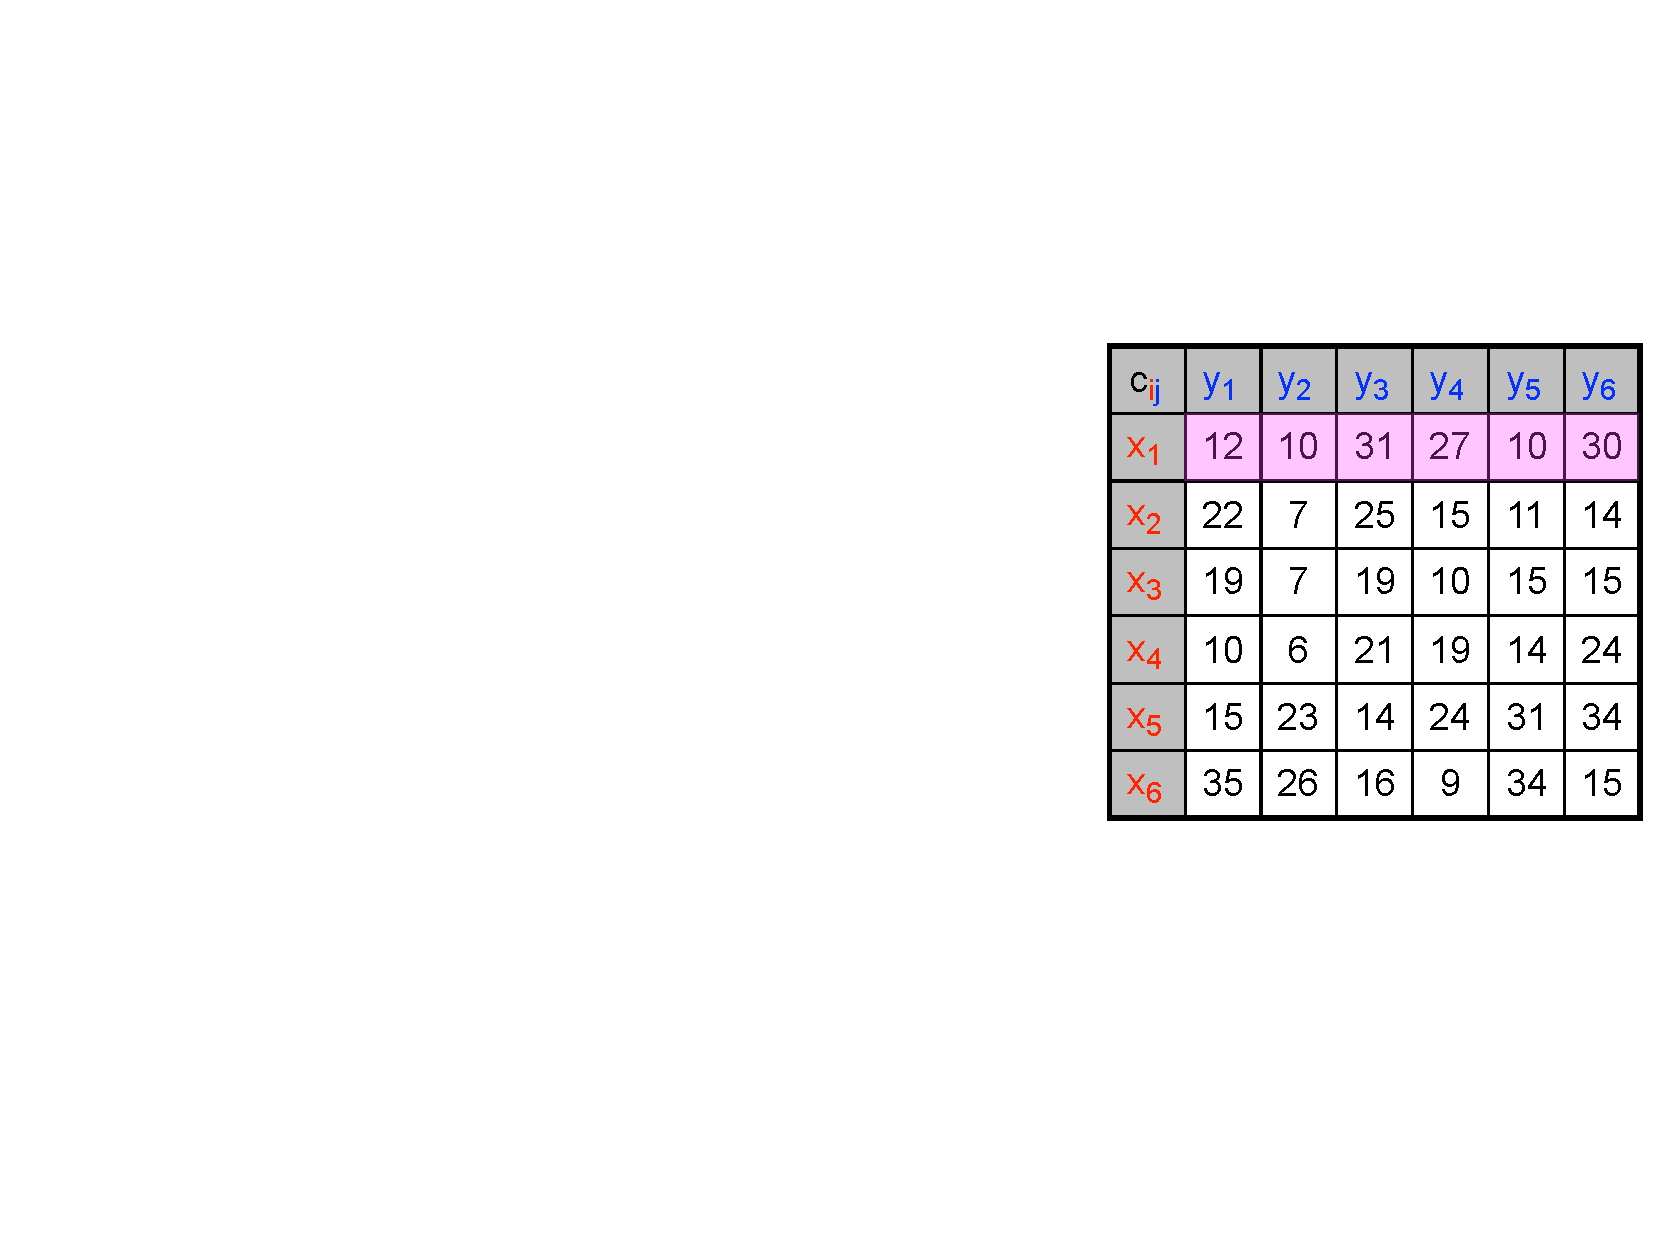
\includegraphics[width=.22\linewidth]{transport/cafe-paris/map-paris-0-couts} 
        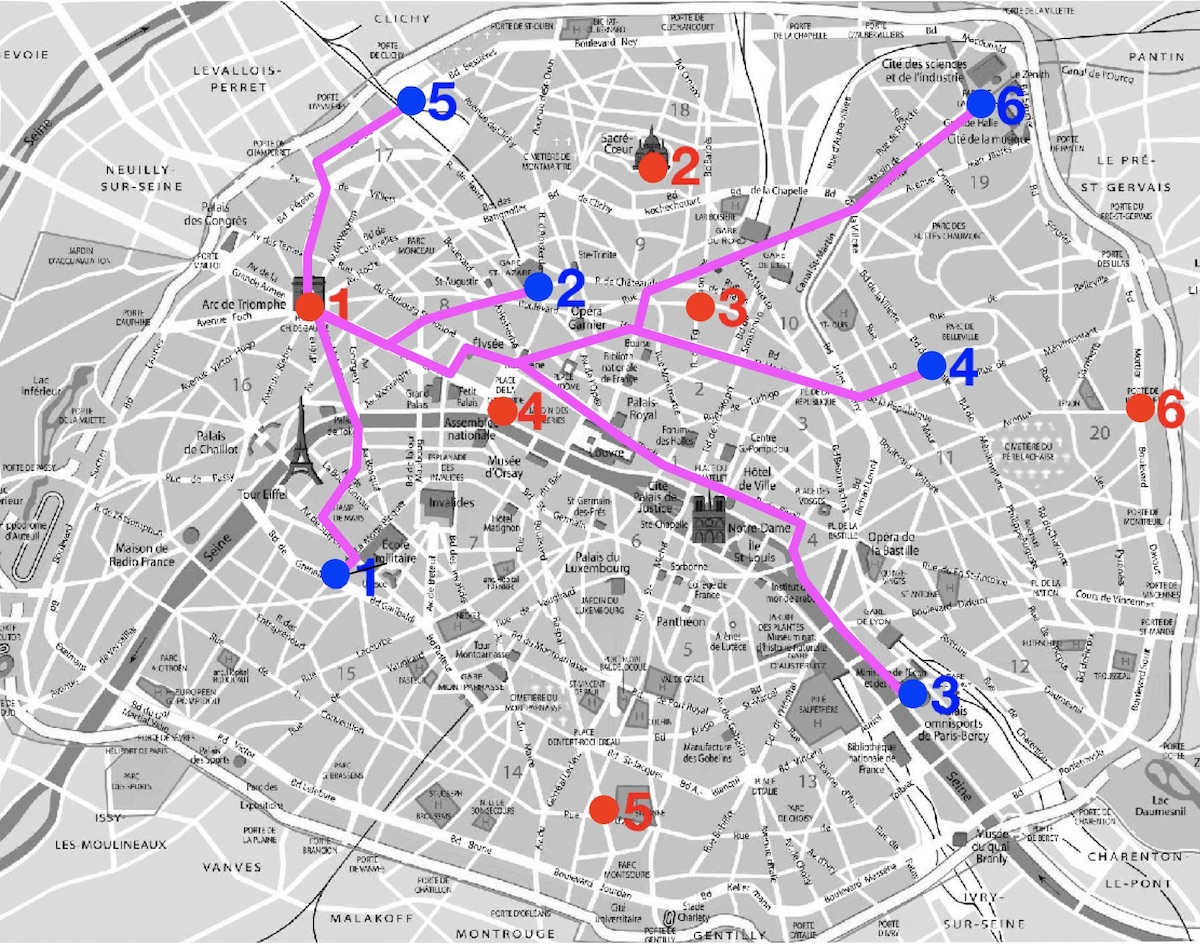
\includegraphics[width=.27\linewidth]{transport/cafe-paris/map-paris-0} 
        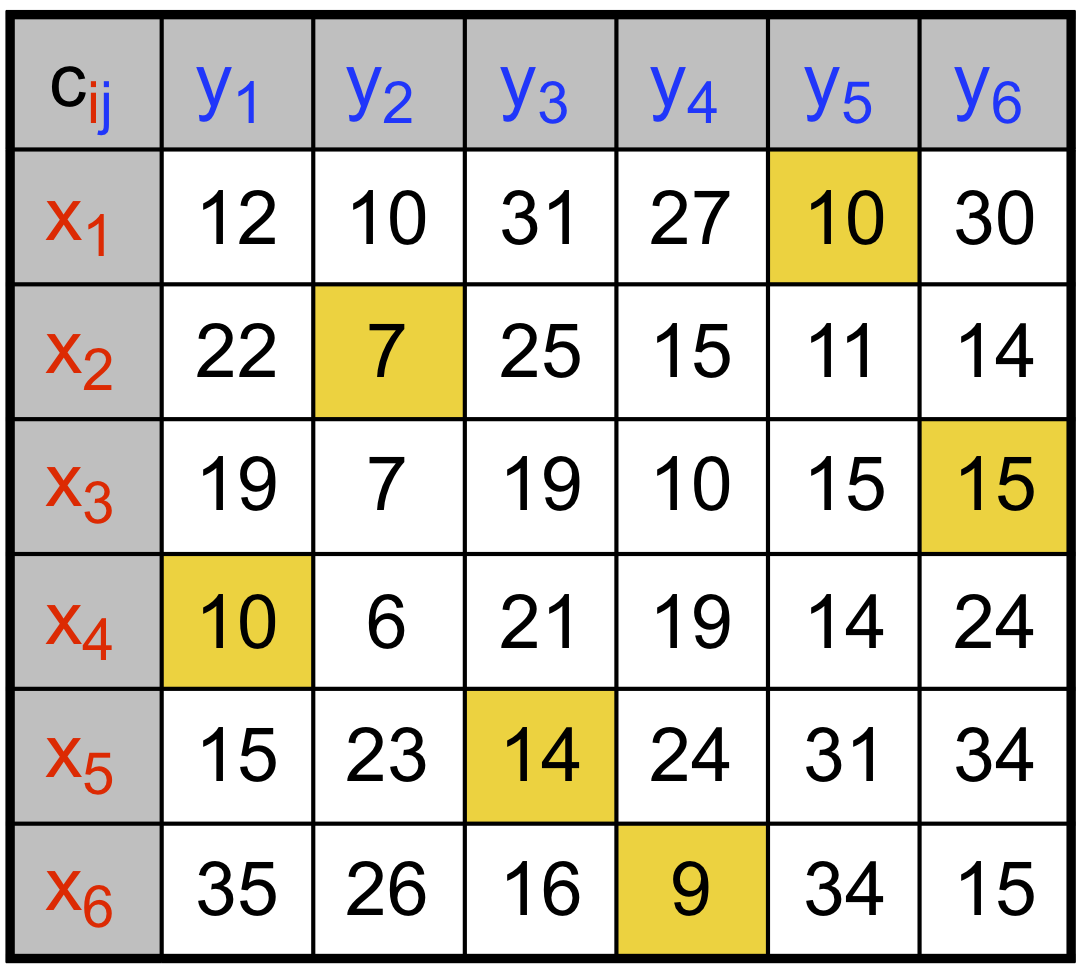
\includegraphics[width=.22\linewidth]{transport/cafe-paris/map-paris-1-couts} 
        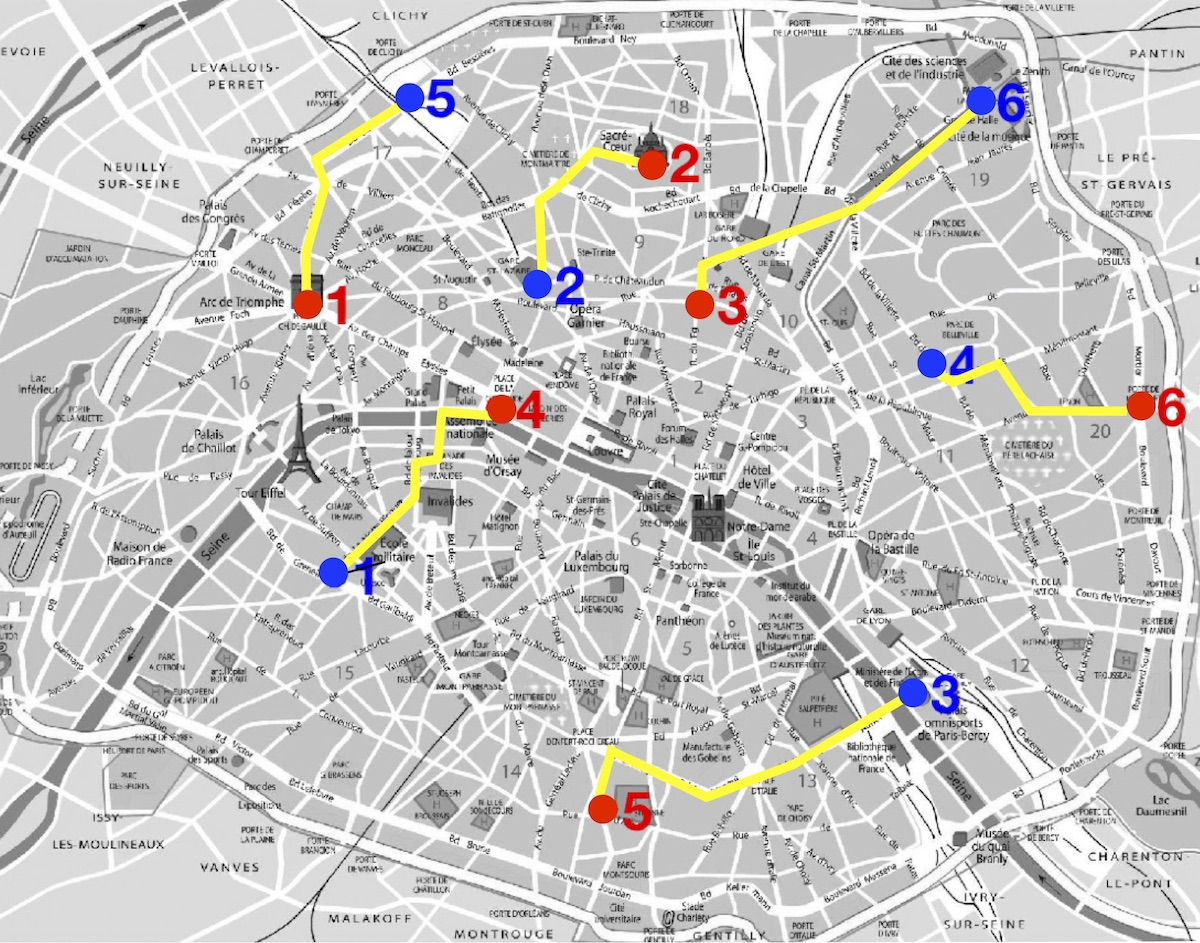
\includegraphics[width=.27\linewidth]{transport/cafe-paris/map-paris-1} 
    \end{tabular}
    \caption{\label{fig:image-cafe} 
    Cost matrix and associated connections. Left: a row of the cost matrix. Right: a particular example of permutation. } 
\end{figure}

In order to meet the supply constraint (also known as mass conservation), each bakery must be connected to one and only one caf\'e. As there are the same number of bakeries as caf\'e, this implies that each caf\'e is also connected to one and only one bakery. We will note
\eq{
    \si: \iC \in \{1, \ldots, 6\} \longmapsto \jC \in \{1, \ldots, 6\}
}
such a choice of connections. Figure~\ref{fig:image-cafe} illustrates in the center and on the right the example
\eql{\label{eq-bijection-exmp}
    \si(\Red{1}) = \Blu{5}, \;
    \si(\Red{2}) = \Blu{2}, \;
    \si(\Red{3}) = \Blu{6}, \;
    \si(\Red{4}) = \Blu{1}, \;
    \si(\Red{5}) = \Blu{3}, \;
    \si(\Red{6}) = \Blu{4}.
}
The mass conservation constraint means that $\si$ is a bijection of the set $\{1, \ldots, 6\}$ within itself. We also say that $\si$ is a permutation.

The transport cost associated with such a bijection is the sum of the costs $C_{\iC, \si (\iC)}$ selected by the permutation $\si$, that is to say
\eql{\label{eq:cout}
    \text{Cost} (\si) \eqdef
        C_{\Red{1}, \si(\Red{1})} +
        C_{\Red{2}, \si(\Red{2})} +
        C_{\Red{3}, \si(\Red{3})} +
        C_{\Red{4}, \si(\Red{4})} +
        C_{\Red{5}, \si(\Red{5})} +
        C_{\Red{6}, \si(\Red{6})}.
}
For example, for the bijection~\eqref{eq-bijection-exmp} shown in Figure~\ref{fig:image-cafe}, we obtain as cost
\eq{
    C_{\Red{1}, \Blu{5}} +
    C_{\Red{2}, \Blu{2}} +
    C_{\Red{3}, \Blu{6}} +
    C_{\Red{4}, \Blu{1}} +
    C_{\Red{5}, \Blu{3}} +
    C_{\Red{6}, \Blu{4}} =
    10 + 7 + 15 + 10 + 14 + 9 = 65.
}


Monge's problem is to look for the permutation $\si$ which has the minimum cost, that is to solve the optimization problem
\eql{\label{eq:monge}
    \umin{\si \in \Si_6} \text{Cost} (\si),
}
where we noted $\Si_6 $ the set of permutations of the set $\{1, \ldots, 6\}$.

\begin{figure}\centering
    \begin{tabular}{@{}c@{\hspace{1mm}}c@{\hspace{1mm}}c@{\hspace{1mm}}c@{}}
        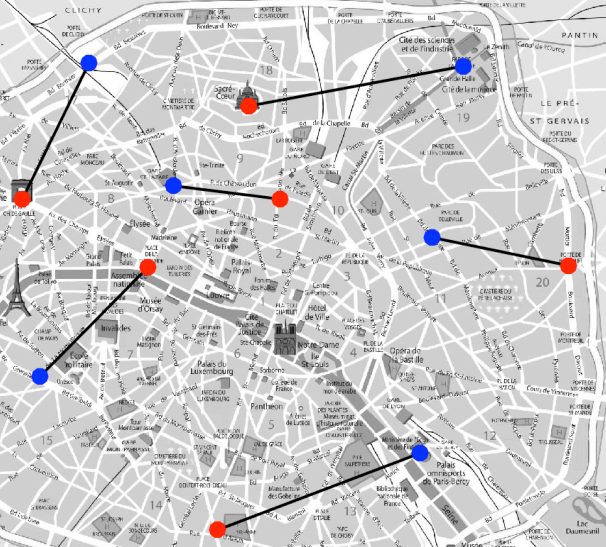
\includegraphics[width=.22\linewidth]{transport/cafe-paris/ordre-croissant-64}&
        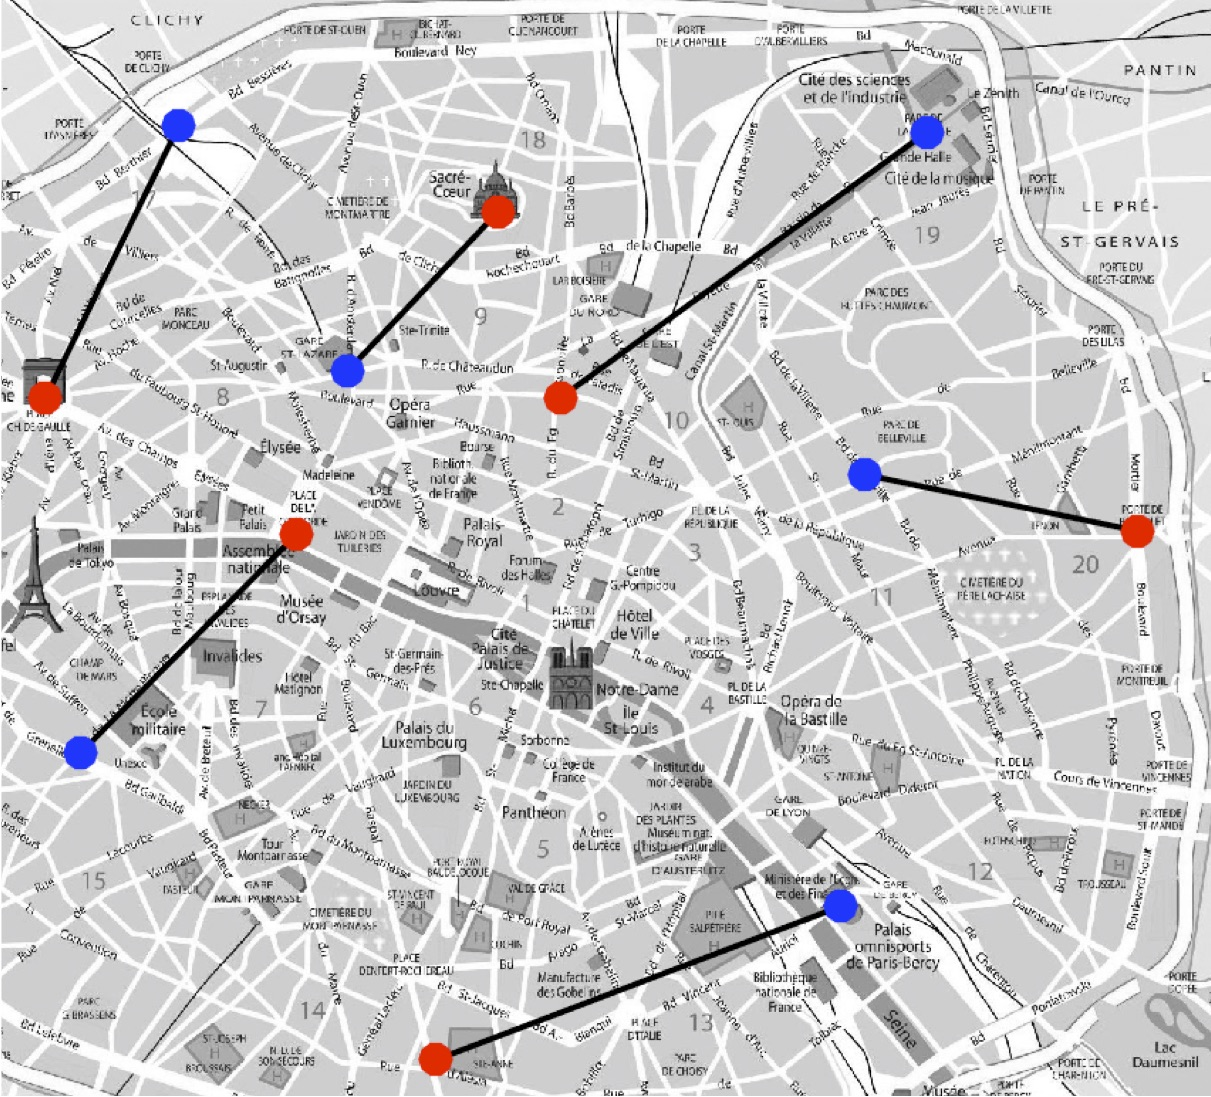
\includegraphics[width=.22\linewidth]{transport/cafe-paris/ordre-croissant-65}&
        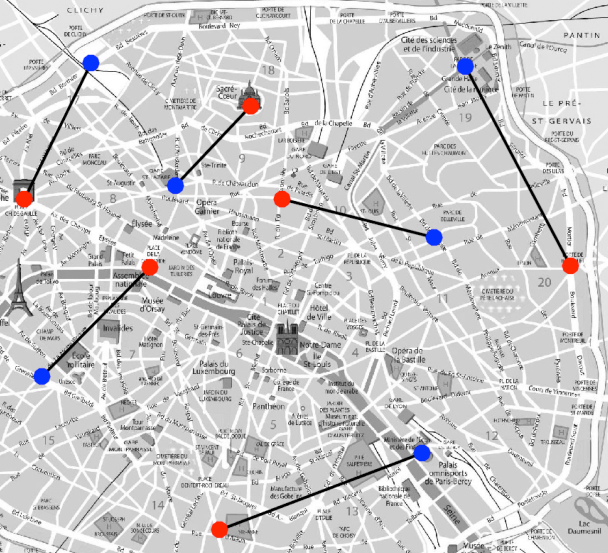
\includegraphics[width=.22\linewidth]{transport/cafe-paris/ordre-croissant-66}&
        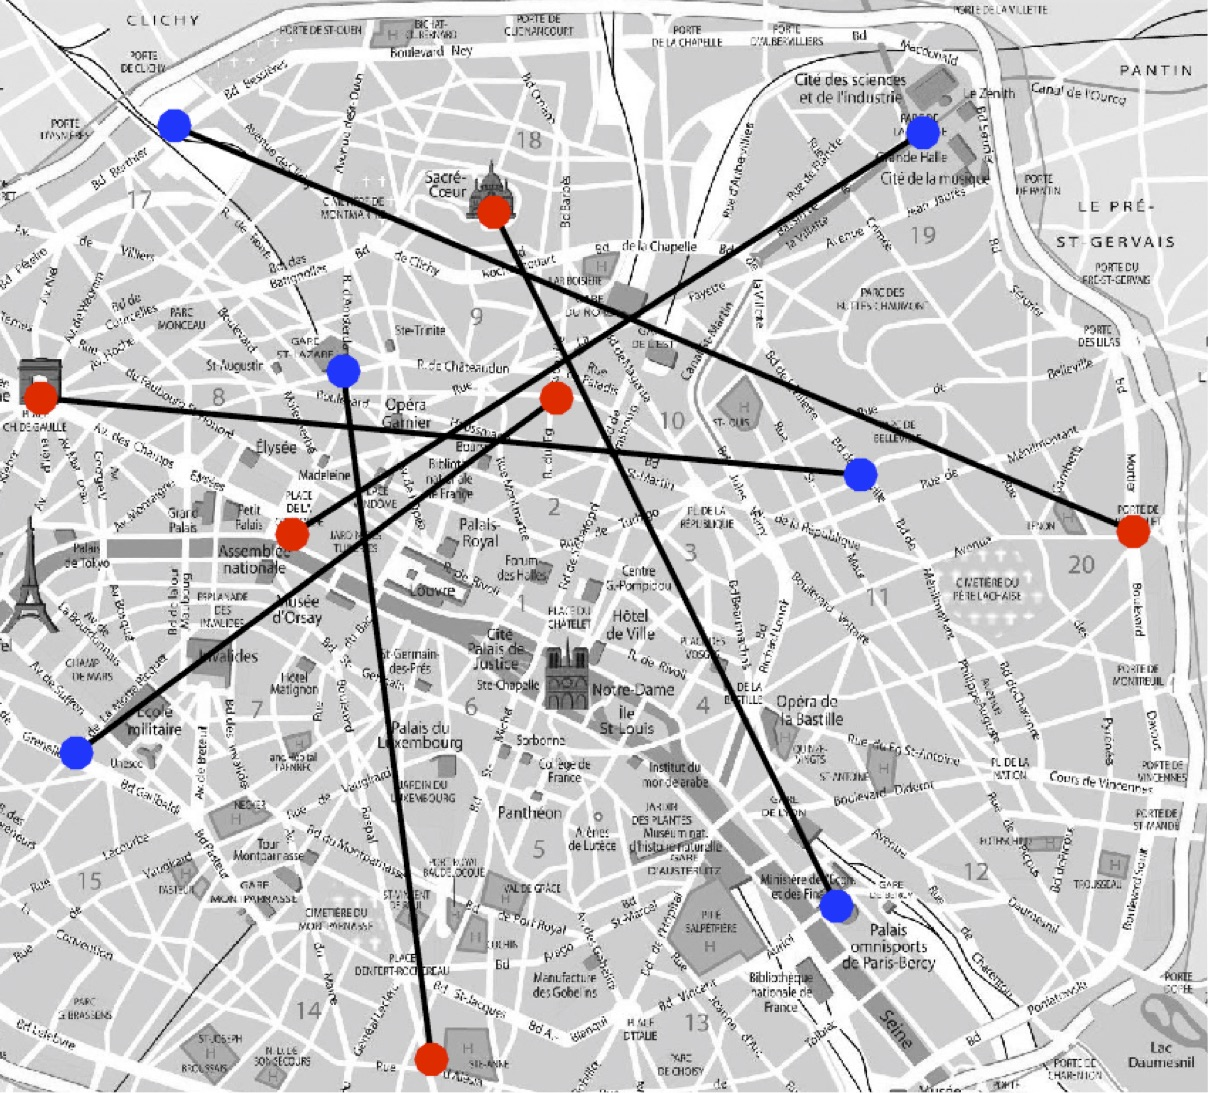
\includegraphics[width=.22\linewidth]{transport/cafe-paris/ordre-croissant-152}\\
        Cost=64 &  
        Cost=65 &  
        Cost=66 &  
        Cost=152
    \end{tabular}
    \caption{\label{fig:order-increasing} Examples of permutations with different costs.
    } 
\end{figure}

Figure~\ref{fig:order-increasing} shows that the permutation~\eqref{eq-bijection-exmp} is not the best: there exists for example another permutation which has a cost of 64. But is this the best? It turns out that it is the case, since we can indeed test on a computer all the permutations of $\{1, \ldots, 6\}$ and calculate their cost. How many permutations are there in total? To make this count, we see that there are six possible assignment choices from $\Red{1}$ to $\si (\Red{1}) \in \{\Blu{1, \ldots, 6 }\}$, then five possible choices to assign $\Red{2}$ to $\si (\Red{2}) \in \{\Blu{1, \ldots, 6}\} - \{\si(\Red{1})\}$, and so on. The total number of possibilities is thus $6 \times 5 \times 4 \times 3 \times 2 \times 1 = 720$ that we note $6!$, \guill{factorial 6}. If we consider a number $n$ of bakeries, then the number of permutations to test to find the best is $n! = n \times (n-1) \times \ldots \times 2 \times 1$. This number grows extremely fast with $n$, for example $70! \approx 1.198 \times 10^{100}$, to be compared with the $10^{11}$ neurons in the brain and the $10^{79}$ atoms in the universe. This exhaustive search strategy is only possible for very small values of $n$.

\begin{figure}\centering
    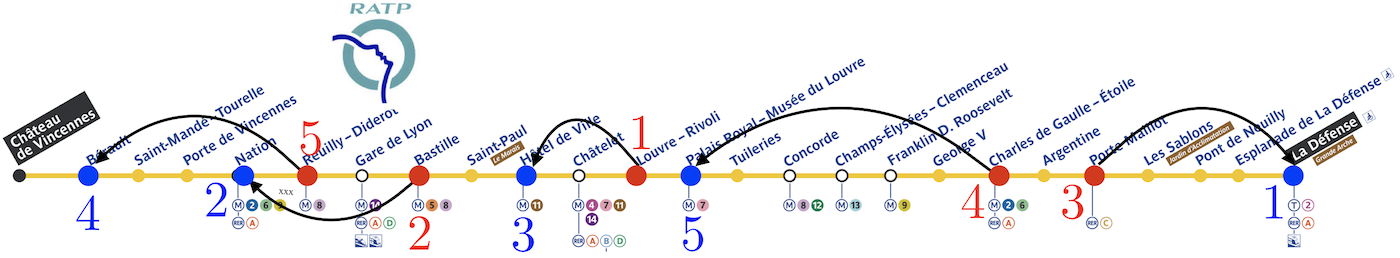
\includegraphics[width=.7\linewidth]{transport/metro/plan-metro}
    \caption{\label{fig:metro} Optimal transport in 1D along a metro line. The optimal bijection is  
    $\si : (\Red{1,2,3,4,5}) \mapsto (\Blu{3,2,1,5,4})$. } 
\end{figure}


%%%%%%%%%%%%%%%%%%%%%%%%%%%%%%%
\myparagraph{In 1D and 2D}

Section~\ref{sec-kanto} explains how mathematical advances have made it possible to develop efficient techniques for calculating an optimal transport $\si$ even for large values of $n$. But it took almost 200 years to get there. In some simple cases, however, the optimal transport can be calculated in a simple way. The most basic case is when the points to be matched are along a 1D axis, for example if caf\'es and bakeries are located along a subway line. It is also necessary that the cost $C_{\iC, \jC}$ be the distance along this axis (eg the metro travel time between the stations). In this case, simply rank the indices $\iC$ and $\jC$ in ascending order (thus from left to right along the subway line) and match the first index $\iC$ to the first index $\jC$ together, then the second index, etc. This process is illustrated in Figure~\ref{fig:metro}. The calculation time required to calculate the optimal transport by subway is therefore the time required to classify the indices. The simplest algorithm for ranking is the one usually used to sort a set of $n$ cards: it is the insertion sort, which iteratively inserts each card in its place relative to the cards already classified. It performs $n(n-1)/2$ comparisons. For $n=70$, this requires only 21415 operations, which makes the method usable, unlike the exhaustive search of all $n!$ Permutations.
%
There are even faster algorithms (eg merge sort), which perform on the order of $n\log(n)$ operations, and hence for $n=70$, such methods require less than 1000 operations.


\begin{figure}\centering
    \begin{tabular}{@{}c@{\hspace{6mm}}c@{\hspace{3mm}}c@{}} % c@{\hspace{1mm}}
        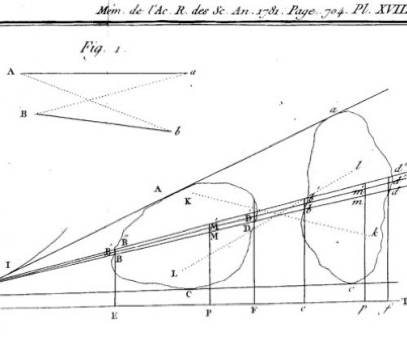
\includegraphics[width=.22\linewidth]{transport/monge-2d/article-monge}&
%        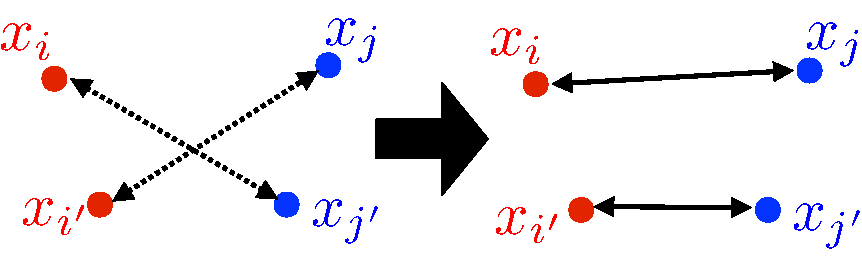
\includegraphics[width=.22\linewidth]{transport/monge-2d/decroisement}&
        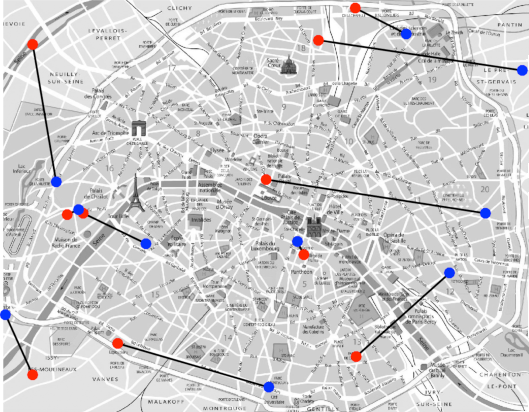
\includegraphics[width=.22\linewidth]{transport/monge-2d/example-10}&
        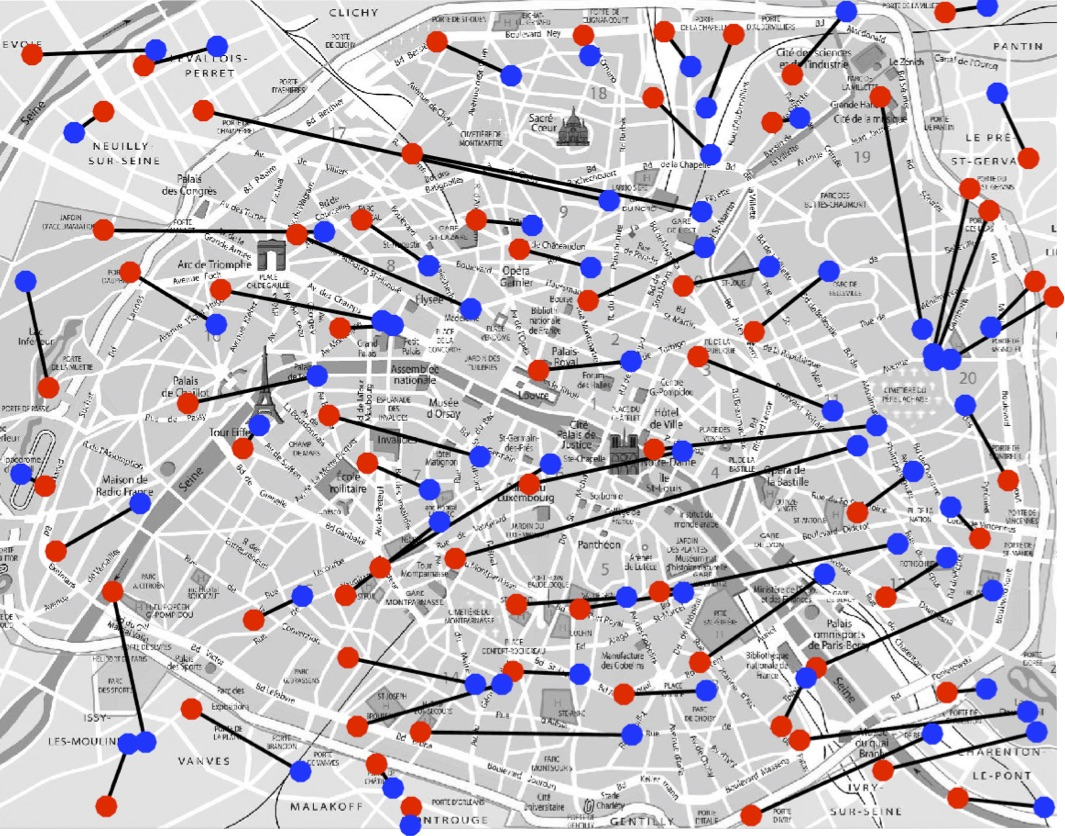
\includegraphics[width=.22\linewidth]{transport/monge-2d/example-70}
    \end{tabular}
    \caption{\label{fig:ot2d} Left: excerpt from Monge's article~\cite{Monge1781}. Right: the optimal transport in 2D for a Euclidean cost.  } 
\end{figure}


Unfortunately, it is no longer possible to use this sorting technique in more general cases. For points in dimension 2, if we take as cost $C_{\iC, \si (\iC)}$  the Euclidean distance (the flight distance) between the points, then Gaspard Monge showed in his paper original (see Figure~\ref{fig:ot2d}, left) that optimal transport can not contain crossover. For example, as shown in Figure~\ref{fig:ot2d} (on the right), if we trace all the segments between the points $\iC \mapsto \jC = \si (\iC)$ that the we connect by the bijection defined by an optimal $\si$, these never cross each other. 
%
This geometrical observation is however not sufficient to compute an optimal transport in 2D: there are indeed many permutations $\si$ such that the associated segments do not intersect.
%
It will be necessary to analyze more finely the structure of the optimal permutations in order to be able to calculate them in an efficient way.
%
We will now see how Leonid Kantorovich has reformulated the problem of Monge in order to achieve this.


%%%%%%%%%%%%%%%%%%%%%%%%%%%%%%%%%%%%%%%%%%%%%%
\section{Optimal Transport of Kantorovich}
\label{sec-kanto}

Leonid Kantorovitch is a Soviet mathematician and economist who revolutionized the theory of optimal transport during the 1940s. His research stemmed from practical considerations that occupied him before and after the Second World War. He played an important role in ensuring an optimal distribution of resources, especially during the Leningrad siege.
%
At the same time, he has been involved in the development of modern optimization, which has had a huge impact in a large number of applied fields. He obtained the Nobel Prize in Economics in 1975, because the first applications (but certainly not the only!) of his theory have been in this field.


%%%%%%%%%%%%%%%%%%%%%%%%%%%%%%%
\myparagraph{Kantorovich's Problem}

Kantorovich's central idea is to modify Monge's problem by replacing the set of permutations with a larger but simpler set. First we notice that we can represent a permutation $\si \in \Si_n$ using a permutation matrix $P$ which is a binary matrix (filled with 0 and 1) of size $n \times n$ such that $P_{\iC, \jC} = 0$ unless $\jC = \si (\iC)$ in which case $P_{\iC, \si (\iC)} = 1$. For example, for $n = 3$ points, the permutations
$(\Red{1,2,3}) \mapsto (\Blu{1,2,3})$ (the identity),
$(\Red{1,2,3}) \mapsto (\Blu{3,2,1})$ and
$(\Red{1,2,3}) \mapsto (\Blu{2,1,3})$ are represented by size $3 \times 3$ matrices
\eq{
\begin{pmatrix} 1 & 0 & 0 \\0 & 1 & 0 \\0 & 0 & 1 \end{pmatrix}, \quad
\begin{pmatrix} 0 & 0 & 1 \\0 & 1 & 0 \\1 & 0 & 0 \end{pmatrix} \qandq
\begin{pmatrix} 0 & 1 & 0 \\1 & 0 & 0 \\0 & 0 & 1 \end{pmatrix}.
}
In the following, $\Pp_n$ is the set of $n!$ Permutation matrices of size $n \times n$.

Since the matrix is binary, with only $n$ non-zero elements equal to 1, we can replace the sum of $n$ terms that appears in $\text{Cost}(\si)$ defined in~\eqref{eq:cout} by a sum over the set of $n \times n$ indices $(\iC, \jC)$, that is, if $P$ is the permutation matrix associated with $\si$, we have
\eq{
	\text{Cost}(\si) = \sum_{\iC = 1}^n \sum_{\jC = 1}^n P_{\iC, \jC} C_{\iC, \jC}.
}
We can thus replace the problem of Monge~\eqref{eq:monge} by the equivalent problem
\eql{\label{eq:mongematrix}
    \umin{P \in \Pp_n} \sum_{\iC = 1}^n \sum_{\jC = 1}^n P_{\iC, \jC} C_{\iC, \jC}.
}

Kantorovich's genius has been to remark that we can replace the discrete set $\Pp_n$ (that is to say composed of a finite, but very large, set of $n!$ Matrices) by a set which is \guill{continuous}  (so in particular infinite) but which is simpler. Note that the permutation matrices of $\Pp_n$ are exactly the matrices that have one and only one along each row and column. This can also be expressed as the fact that a permutation matrix is a binary matrix whose sum of each row and of each column is 1, that is to say
\eq{
	\Pp_n = \enscond{P \in \{0,1\}^{n \times n}}{\foralls \iC, \sum_{\jC} P_{\iC, \jC} = 1, \foralls \jC, \sum_{\iC} P_{\iC, \jC} = 1}.
}
What makes this set very complicated is the binary constraint, that is, these matrices are constrained to be in $\{0,1\}^{n \times n}$. Kantorovitch then proposes to \guill{relax} this constraint by simply assuming that the entries of $P$ are between $0$ and $1$. This defines a larger set, the set of bistochastic matrices
\eql{\label{eq:bistoch}
\Bb_n \eqdef \enscond{P \in [0,1]^{n \times n}}{\foralls \iC, \sum_{\jC} P_{\iC, \jC} = 1, \foralls \jC, \sum_{\iC} P_{\iC, \jC} = 1}.
}
The Kantorovitch problem is obtained by performing this replacement in~\eqref{eq:mongematrix}, in order to solve
\eql{\label{eq:kantoassign}
    \umin{P \in \Bb_n}
        \sum_{\iC = 1}^n \sum_{\jC = 1}^n P_{\iC, \jC} C_{\iC, \jC}.
}
The huge advantage of the Kantorovich~\eqref{eq:kantoassign} problem over that of Monge~\eqref{eq:mongematrix} is that the set of bistochasic matrices is convex, ie if we consider two bistochasic matrices $P, Q \in \Bb_n$, so their mean $\frac{P + Q}{2} \in \Bb_n$ is still bistochasic. This is not true for permutation matrices, since the average of two binary matrices $(P,Q)$ is not binary (except of course if $P=Q$). This convexity is the key to the development of efficient algorithms.
%
This new formulation has indeed benefited from a second revolution initiated by George Dantzig~\cite{Dantzig51}, which, at the same time, proposed the algorithm of the simplex. This one allows to solve efficiently a certain class of convex optimization problems: linear programming problems, of which~\eqref{eq:kantoassign} is a particular case. In the case of the Kantorovitch problem, there is indeed a simplex algorithm that has a complexity of the order of $n^3$ operations, which allows calculations to be made for large $n$, of the order several thousands.


%%%%%%%%%%%%%%%%%%%%%%%%%%%%%%%
\myparagraph{Monge--Kantorovich Equivalence}

The set of bistochastic matrices is larger than the set of permutations matrices, $\Pp_n \subset \Bb_n$, so that we have the inequality
\eql{\label{eq:monge-vs.-Kanto}
    \umin{P \in \Bb_n}
        \sum_{\iC = 1}^n \sum_{\jC = 1}^n P_{\iC, \jC} C_{\iC, \jC}
     \leq
    \umin{P \in \Pp_n}
        \sum_{\iC = 1}^n \sum_{\jC = 1}^n P_{\iC, \jC} C_{\iC, \jC}
}
between the problems of Kantorovich and Monge. But a fundamental theorem due to George Birkhoff and John von Neumann~\cite{birkhoff,von1953certain} ensures that in fact there is equality between the values of these two minimizations. Indeed, this theorem shows that there is always a solution matrix of the Kantorovitch problem which is a matrix of permutation, so that it is also a solution to Monge's problem. Beware however, in general there is no uniqueness of the solutions of these problems: there may exist a bistochastic matrix solution of the Kantorovich problem which is not a permutation.
%
The combination of two spectacular advances, due to Kantorovich and Dantzig, made optimal transport applicable to large scale problems, since the simplex algorithm can be used to solve these problems in practice.

%%%%%%%%%%%%%%%%%%%%%%%%%%%%%%%
\myparagraph{The Weighted Case}

In addition to its practical interest, Kantorovich's formulation has also allowed generalizing Monge's initial problem, by giving the right framework to formalize it and study it mathematically. Indeed, Monge's problem is quite limited. What happens for example if there is not the same number $n$ caf\'e and $m$ bakeries? The initial problem~\eqref{eq:monge} has no solution, because you can not put in bijection two sets of different sizes. The right concept is not the number of bakeries and caf\'es, but rather the $(\Red{a_1, \ldots, a_n})$ production distributions (associated with bakeries) and the $(\Blu{b_1, \ldots, b_m})$ of caf\'e consumption.
%
For example, if the first bakery produces 45 croissants a day, we will take $\Red{a_1}=45$, and $\Blu{b_3}=34$ means that the $3^\text{rd}$ caf\'e consumes 34 croissants a day.
%
In the case initially considered, where $n=m$, all the quantities $\Red{a_i}$ and $\Blu{b_j}$ are equal to 1. But in many concrete cases, these quantities are arbitrary. These quantities must be positive, and satisfy
\eq{
\Red{a_1 + \cdots + a_n} = \Blu{b_1 + \cdots + b_m},
}
so that there is as much production as consumption. Kantorovich's construction naturally adapts to this case of general distributions, replacing the bistochasic matrices~\eqref{eq:bistoch} by matrices of \guill{coupling} which satisfy the mass conservation constraint.
\eq{
\Bb(\aC, \bC) \eqdef \enscond{P \in [0,1]^{n \times m}}{\foralls \iC, \sum_{\jC} P_{\iC, \jC} = \Red{a_i}, \foralls \jC, \sum_{\iC} P_{\iC, \jC} = \Blu{b_j}}.
}
In the original case $n=m$ and $\Red{a_i} = \Blu{b_j} = 1$, then $\Bb(\aC, \bC) = \Bb_n$ which corresponds to doubly stochastic matrices. In the general case, whenever an entry $P_{\iC, \jC}$ is non-zero, this means that there is some transfer of \guill{mass} (here a certain amount of croissants) between $\iC$ and $\jC$. As shown in Figure~\ref{fig:coupling-visu}, we can visualize in different ways such a matrix $P$ coupling two distributions $(\aC, \bC)$.
%
Unlike the case of doubly stochastic matrix, for which there is always a solution that is a permutation, here optimum coupling $\Bb(\aC, \bC)$ can have more than one non-zero entry $P_{\iC,\jC}$ along a line indexed by $\iC$ (see Figure~\ref{fig:coupling-visu}). This means that this bakery $\iC$ is connected to several caf\'es, so that its production is then separated into several  batches distributed while meeting conservation constraint of the mass $\sum_{\jC} P_{\iC \jC} = \Red{a_i}$.

\begin{figure}\centering
    \begin{tabular}{@{}c@{\hspace{1mm}}c@{\hspace{1mm}}c@{\hspace{1mm}}c@{}}
        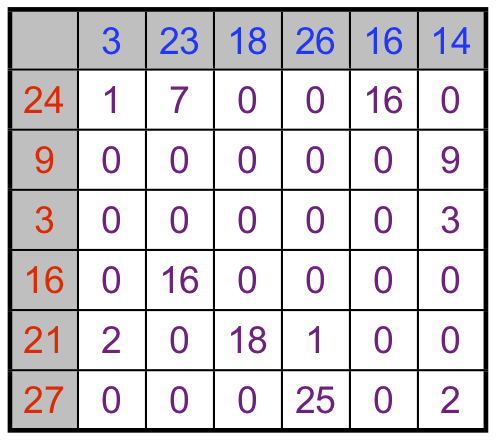
\includegraphics[width=.22\linewidth]{transport/kantorovitch/coupling-array}&
        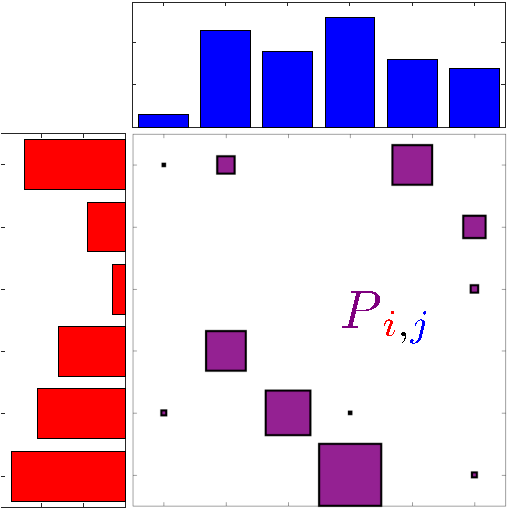
\includegraphics[width=.22\linewidth]{transport/kantorovitch/coupling-squares}&
        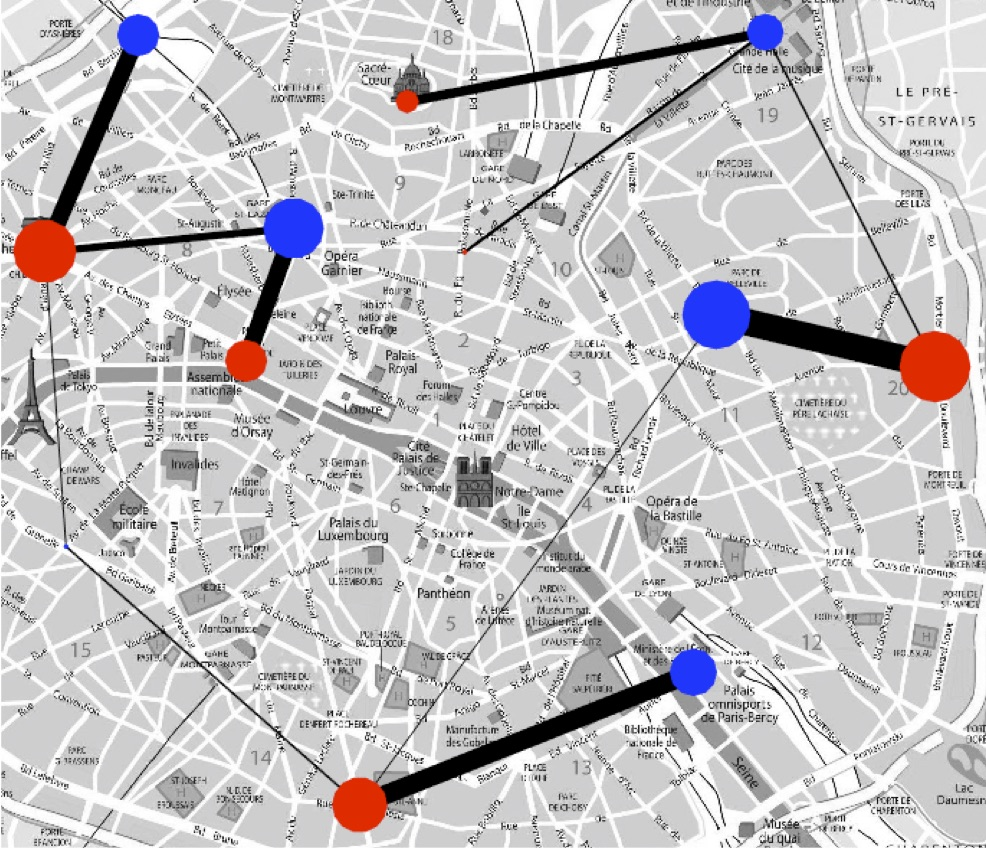
\includegraphics[width=.22\linewidth]{transport/kantorovitch/coupling-map}&
        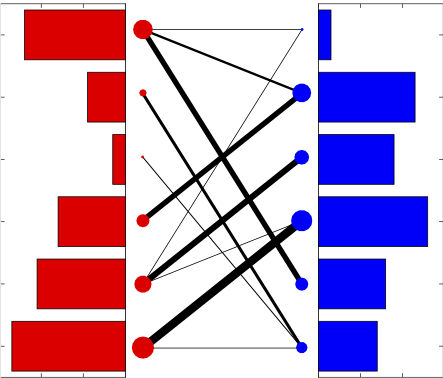
\includegraphics[width=.22\linewidth]{transport/kantorovitch/coupling-bipartite} \\
        (a) matrix & (b) histograms & (c) segments & (d) bipartite graph
    \end{tabular}
    \caption{\label{fig:coupling-visu} Different ways of representing a coupling matrix $P \in \Bb(\aC, \bC)$:
    (a) a table of numbers whose rows and columns have prescribed sums;
(b) a two-dimensional histogram whose square size is propositional to $P_{\iC, \jC}$;
(c) a set of segments whose width is proportional is $P_{\iC, \jC}$.
(d) a bipartite graph, that is to say with two sets of vertices such that the edges are only between these two sets.  } 
\end{figure}


Kantorovich's problem which generalizes~\eqref{eq:kantoassign} is then written
\eql{\label{eq-kanto-gen}
    \umin{P \in \Bb (\aC, \bC)}
        \sum_{\iC = 1}^n \sum_{\jC = 1}^m P_{\iC, \jC} C_{\iC, \jC}
}
which means that you have to pay $C_{\iC, \jC}$ each time you transfer a unit of mass between $\iC$ and $\jC$. Just like the original problem~\eqref{eq:kantoassign}, we can solve it effectively with the simplex algorithm. Figure~\ref{fig:coupling-visu} shows an example of optimal coupling. 



%%%%%%%%%%%%%%%%%%%%%%%%%%%%%%%%%%%%%%%%%%%%%%
\section{Applications}

Although the initial motivations of Monge and Kantorovitch were respectively military and economic, the optimal transport finds countless applications, both theoretical but also more concrete. Mathematically, one can consider \guill{continuous} distributions of masses, somehow the limit when the number of point $n$ tends to infinity. This makes it possible to define the transport problem between any probability measurements. This theoretical point of view is extremely fruitful, and it was the French mathematician Yann Brenier who first showed equivalence in the continuous framework of the formulations of Monge and Kantorotich~\cite{Brenier91}. These pioneering works showed the connection between the transport problem and the partial differential equations, and led, among other things, to the Fields medals of Cédric Villani (2010) and Alessio Figalli (2018).

\begin{figure}\centering
\begin{tabular}{@{}c@{\hspace{1mm}}c@{\hspace{1mm}}c@{}}
    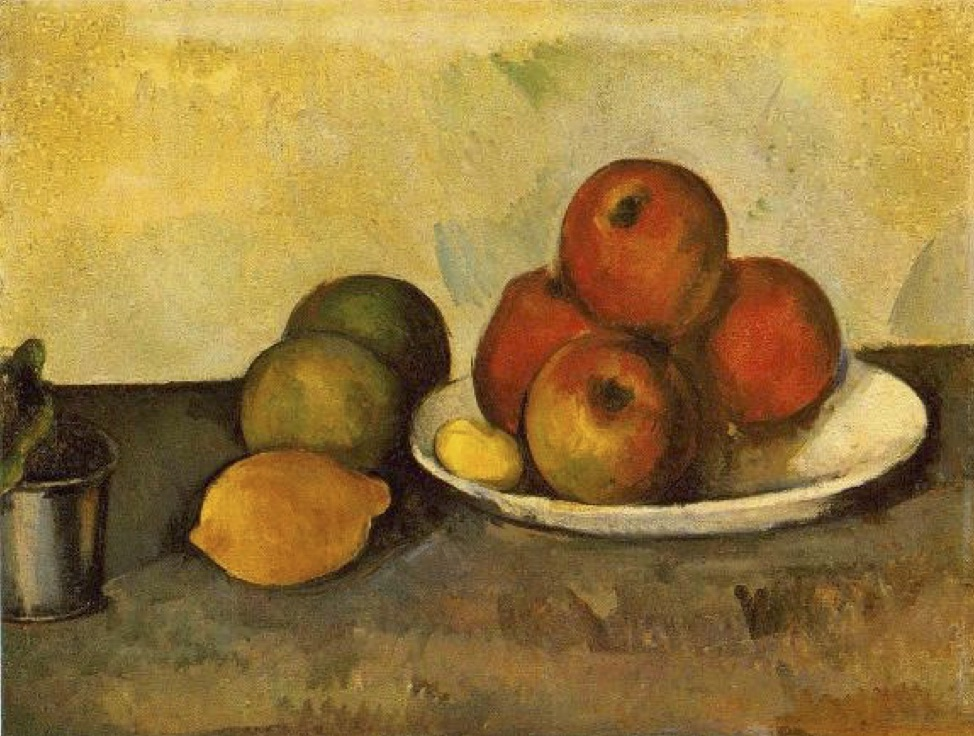
\includegraphics[width=.24\linewidth]{transport/applis/painting-2} &
    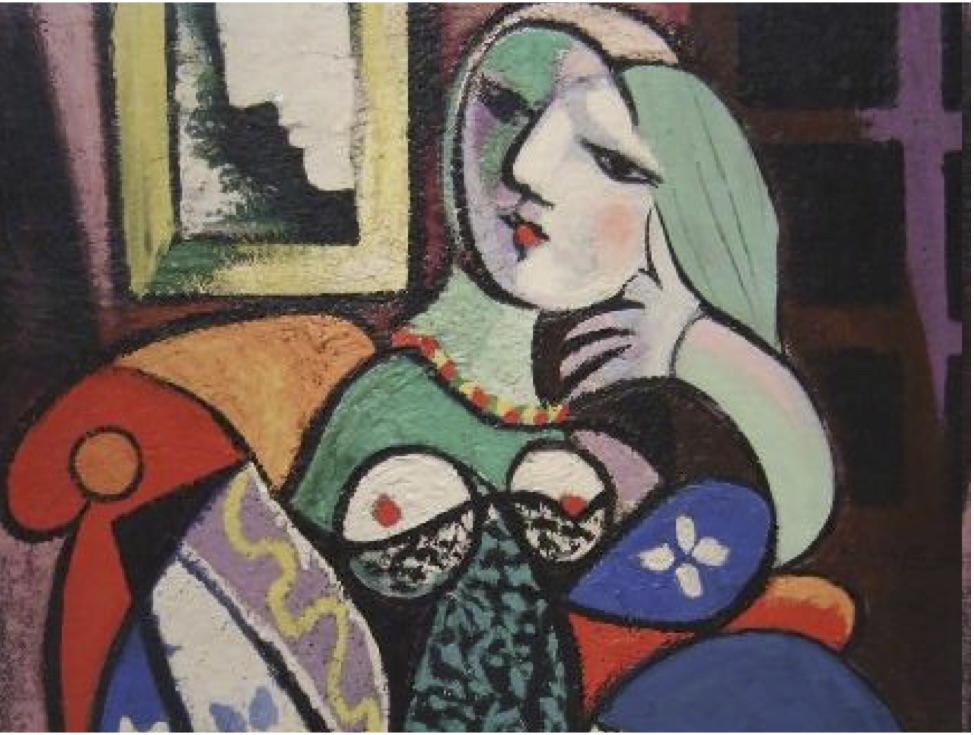
\includegraphics[width=.24\linewidth]{transport/applis/painting-1} &
    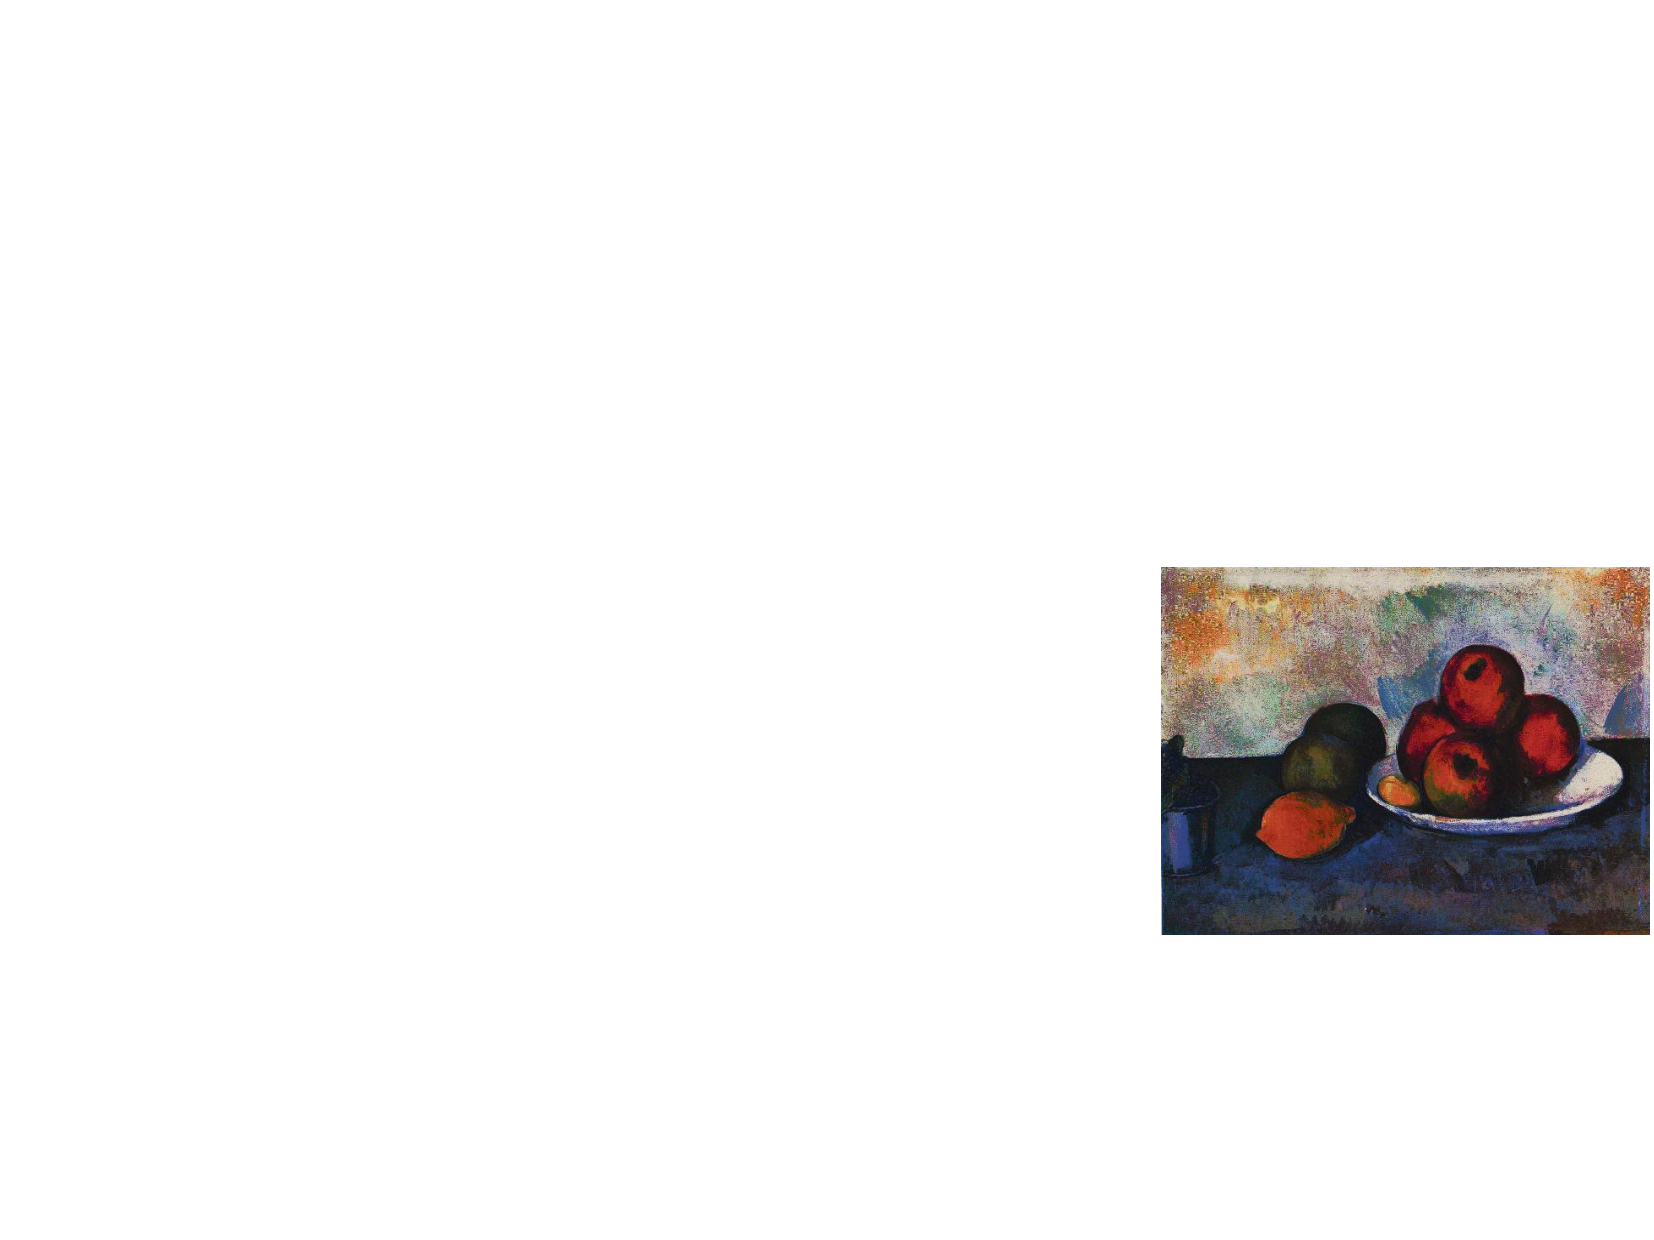
\includegraphics[width=.24\linewidth]{transport/applis/painting-2-equalized} \\
    Image $(\Red{x_i})_{\iC=1}^n$& Image $(\Blu{y_j})_{\jC=1}^n$& Image  $(y_{\si(\iC)})_{\iC=1}^n$\\
    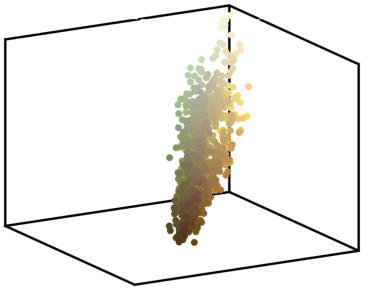
\includegraphics[width=.24\linewidth]{transport/applis/painting-2-histo}&
    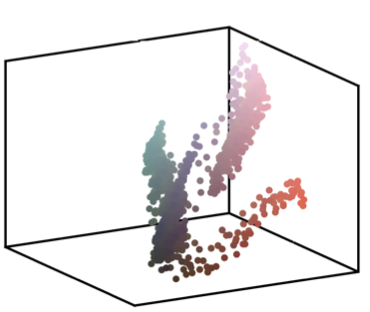
\includegraphics[width=.24\linewidth]{transport/applis/painting-1-histo}&
    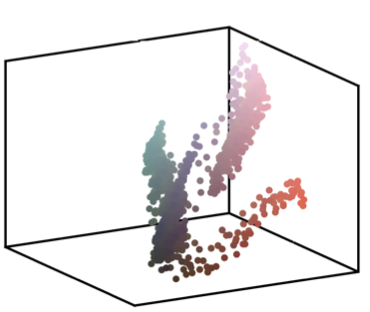
\includegraphics[width=.24\linewidth]{transport/applis/painting-1-histo}
\end{tabular}
\caption{\label{fig:image-eq} 
Example of transferring color palettes using optimal transport.
Top: The pixels are on the display grid to form a color image.
Bottom: The pixels are placed at their positions in $\RR^3$ to form a scatter plot. }
\end{figure}

Optimal transport has recently become the focus of more applied problems in data sciences, especially to solve problems in image processing and machine learning.
%
The first idea, the most immediate, is to use the bijection $\si$ to transform data, for example images. In this case, the pixels $(\Red{x_i})_{\iC = 1}^n$ and $(\Blu{y_j})_{\jC = 1}^n$of two color images are considered. Each pixel $\Red{x_i}, \Blu{y_j} \in \RR^3$ is a vector of dimension 3, which represents the intensities of each of the three elementary colors, red, green and blue. In order to change the colors of the first image, and impose the palette of the second image, we calculate the transport $\si$ for the cost matrix $C_{\iC} = \norm{\Red{x_i} - \Blu{y_j}}^2$ (that is, the square of the Euclidean norm in $\RR^3$), which is the square of the Euclidean distance between the pixels. The image with the modified colors is $(y_{\si (\iC)})_{\iC = 1}^n$, ie we replace in the first image the pixel $\Red{x_i}$ by the pixel $y_{\si(\iC)}$. This image looks like the first, but has the color palette of the second image.
%
Figure~\ref{fig:image-eq} illustrates this process to impose the color palette of Picasso to a painting by Cézanne.

Optimal transport can also be used for more difficult problems, by only indirectly using the bijection $\si$ or the optimal coupling matrix $P \in \Bb(\aC,\bC)$. The central idea is that the quantity associated with an optimal coupling $P$ solution of~\eqref{eq-kanto-gen}
\eq{
	W(\aC, \bC) \eqdef \sum_{i, j} P_{\iC, \jC} C_{\iC, \jC}
}
somehow defines the effort required to move the mass of the $\aC$ distribution to the $\bC$ distribution. It allows to quantify how much these two distributions are \guill{close}. For example, if $C_{\iC,\jC} = \norm{\Red{x_i} - \Blu{y_j}}^2$ is the square of the Euclidean distance between points, then the quantity $W (\aC, \bC)^{1/2}$ is a distance between the distributions, in particular it satisfies $W(\aC, \bC) = 0$ if and only if $\aC = \bC$, and it satisfies the inequality triangular. These properties are very important for applying transport to practical problems.


\begin{figure}\centering
        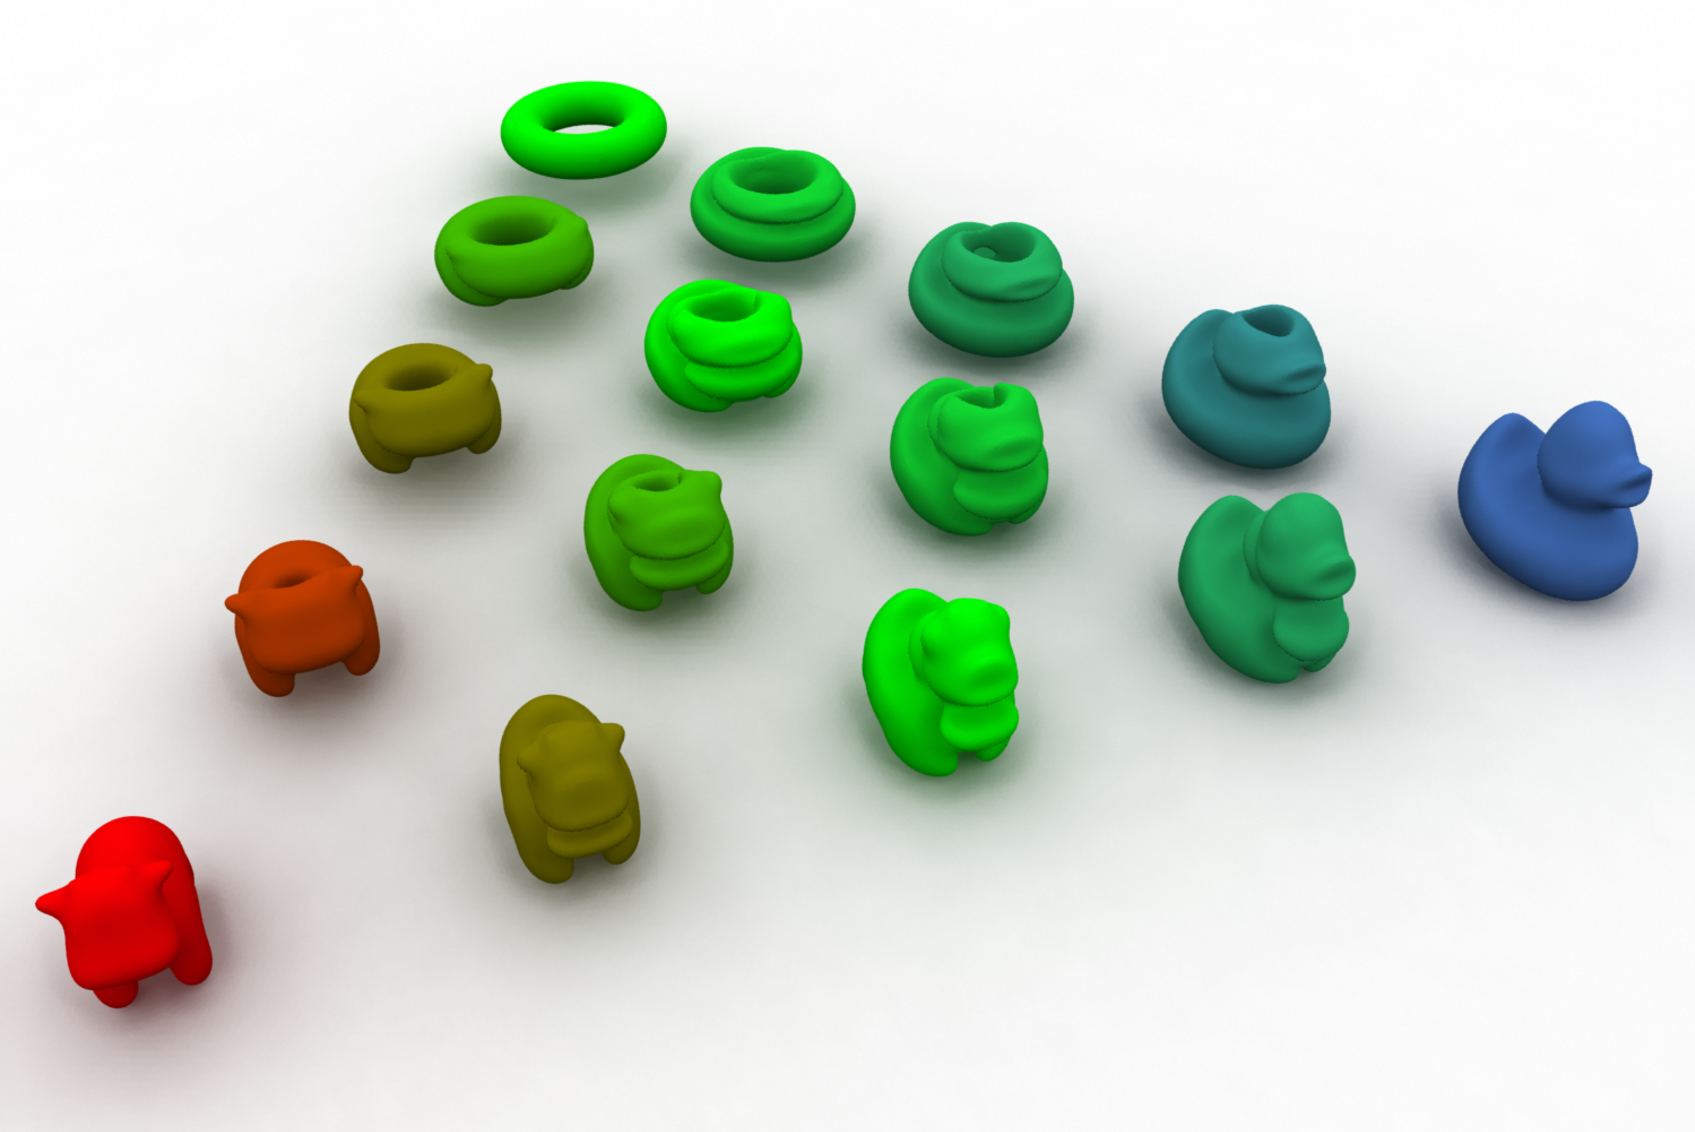
\includegraphics[width=.6\linewidth]{transport/applis/shapes-3d}
    \caption{\label{fig:barycenters} Example of barycentric interpolation between 3D forms, obtained by minimizing~\eqref{eq-bary}.  }
\end{figure}

A typical example of the application of this $W$ quantity is to compute centroids between~\cite{agueh2011barycenters} distributions. Figure~\ref{fig:barycenters} shows an example where we consider three distributions $a, b, c$ (shown at the three vertices of the triangles) which are uniform mass distributions inside 3D shapes (that is, the mass $a_i$ associated with the $i^{\text{th}}$ point is 0 outside the first form and takes a constant value inside).
%
A weighted barycenter of these three distributions is calculated by mimicking the fact that in a Euclidean space, the weighted centroid $r$ of three points $x, y, z$ minimizes the sum of distances squared.
\eq{
    \umin{r} \al \norm{x-r}^2 + \be \norm{y-r}^2 + \ga \norm{z-r}^2,
}
where the weights $(\al, \be, \ga)$ are the weightings of the centroid, which are positive reals and such that $\al + \be + \ga = 1$.
%
The weighted barycenter $d$ of $(a, b, c)$ thus minimizes the weighted sum of optimal transport distances
\eql{\label{eq-bary}
\umin{d} \al W (a, d) + \be W (b, d) + \ga W (c, d).
}
By modifying the weights $(\al, \be, \ga)$, we modify the shape obtained by moving inside an optimal transport triangle.
%
This $W$ distance can be used for many other applications where probability distributions must be compared. This is the case in machine learning, for example to compare texts using the distributions of words that compose them. Figure~\ref{fig:bagwords} illustrates the  histograms of appearance of words for two texts, where the size of the letters of the word $\iC$ is proportional to the mass $\aC_\iC$. A difficult question in this case is which cost matrix $C_{\iC, \jC}$ to use between two words $(\iC, \jC)$. It is a linguistics problem (to characterize the semantic proximity between words of a language), which one can seek to solve at the same time as the optimal transport~\cite{huang2016supervised}.

\begin{figure}\centering
    
\includegraphics[width=.35\linewidth]{transport/applis/bag-word-1}
    \qquad
    
\includegraphics[width=.35\linewidth]{transport/applis/bag-word-2}
\caption{\label{fig:bagwords} Examples of histograms of word distributions in two different texts (only the most frequent words are shown). }
\end{figure}


%%%%%%%%%%%%%%%%%%%%%%%%%%%%%%%%%%%%%%%%%%%%%%
\section*{Conclusion}

Optimal transport has seen many revolutions. Led by mathematicians such as Monge, Kantorovich, Danzig and Brenier, it has gradually become a fundamental theoretical and numerical tool.
%
It is now at the heart of important questions in data science to model, numerically solve and theoretically analyze problems in machine learning. The opportunities to develop new theories and powerful algorithms are immense.
%
For more information on the theoretical aspects of optimal transport, one can consult the books~\cite{Villani03, SantambrogioBook}. Numerical and applicative aspects are covered in the book~\cite{PeyreCuturi}.

%%%%%%%%%%%%%%%%%%%%%%%%%%%%%%%%%%%%%%%%%%%%%%
\section *{Acknowledgments}

I would like to thank Vincent Beck, Gwenn Guichaoua and Marie-Noëlle Peyr\'e for their careful proofreadings.